\section{Proposed Approach}\label{sec:approach}

\subsection{System Architecture}\label{sec:sysarch}

Figure~\ref{fig:sysarch} shows the end-to-end pipeline of the theorem prover.
A problem in the TPTP syntax (.p file) is parsed into an initial
sequent $\Gamma \vdash \Delta$,
with premises on the left and the conjecture on the right.
The sequent is dispatched to one of three engines; each engine injects a
\emph{scheduler policy} into the shared \texttt{backwards\_search} kernel and
optionally wraps it in an iterative-deepening envelope.
The kernel returns one of four outcomes: \textit{Provable}, \textit{NotProvable}
(the goal is counter-satisfiable), \textit{Unknown} (a resource bound was
reached without a decision), or \textit{Timeout}.
All three engines share every component except the injected scheduler and
whether an iterative-deepening loop is present.

\begin{figure}[t]
  \centering
  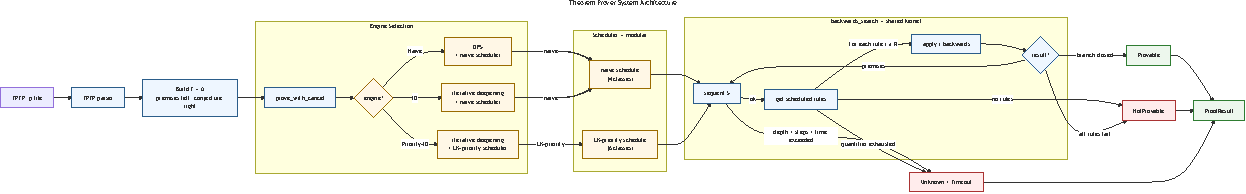
\includegraphics[width=\linewidth]{figures/system_architecture_diagram.pdf}
  \caption{System architecture of the theorem prover. Engine selection
    determines both the search strategy and the injected scheduler;
  \texttt{backwards\_search} is shared across all engines.}
  \label{fig:sysarch}
\end{figure}

\subsection{Baseline: Naive Backward Search}\label{sec:baseline}

Backward proof search applies LK$'$ inference rules \emph{root-first}: the
prover starts from the goal sequent $\vdash A$ and recursively decomposes it
until every open leaf is closed by a \emph{closing rule}: the identity axiom
($\phi \vdash \phi$), $\top R$, or $\bot L$.  Branching rules ($\wedge R$,
$\vee L$, ${\rightarrow}L$) spawn multiple sub-goals that must all close for
the parent to close; non-branching rules produce a single successor.

Quantifier rules divide into two classes with distinct side-conditions.
The \emph{eigenvariable} rules $\forall R$ and $\exists L$ substitute a
fresh constant that does not appear elsewhere in the current sequent,
preserving the eigenvariable condition required for soundness.
The \emph{reusable} rules $\forall L$ and $\exists R$ differ from classical
LK: the original quantified formula is \emph{retained} on the sequent after
instantiation, permitting repeated application with different witness terms.

Algorithm~\ref{alg:naive} reproduces the na\"ive backward proof-search
procedure of Hou~\cite[p.~67]{hou2021fundamentals}, restated in our notation.
Rules are applied in five sequential priority groups: (1)~closing rules;
(2)~invertible propositional rules and eigenvariable quantifiers ($\wedge L$,
$\vee R$, ${\rightarrow}R$, $\neg L$, $\neg R$, $\forall R$, $\exists L$);
(3)~branching propositional rules ($\wedge R$, $\vee L$, ${\rightarrow}L$);
(4)~reusable quantifiers ($\forall L$, $\exists R$) with a visible term not
yet used for that quantified occurrence; and (5)~reusable quantifiers with a
freshly generated witness.  Groups are mutually exclusive: a higher-priority
group is exhausted before any rule from a lower-priority group is tried.

% Requires \usepackage{algorithm} and \usepackage{algpseudocode}.
% This fragment is intended to be included from report/report.tex.
\begin{algorithm}
  \caption{Na\"ive backward proof search for LK$'$ (Algorithm~2 of
  \cite[p.~67]{hou2021fundamentals})}\label{alg:naive}
  \begin{algorithmic}[1]
    \Require First-order formula $A$
    \Ensure Derivation tree in LK$'$, or report no proof found
    \State build the bottom sequent $\vdash A$
    \ForAll{top sequents on an open branch}
    \If{any of $\mathit{id}, \top R, \bot L$ is applicable}
    \State apply the rule backwards and close the branch
    \ElsIf{any of $\wedge L, \vee R, {\rightarrow}R, \neg L, \neg R,
    \forall R, \exists L$ is applicable}
    \State apply the rule backwards
    \ElsIf{any of $\wedge R, \vee L, {\rightarrow}L$ is applicable}
    \State apply the rule backwards and create a new branch
    \ElsIf{$\forall L$ or $\exists R$ is applicable, and there is a
      term $t$ that has not been used to instantiate the quantified
    variable $x$ in this formula}
    \State apply the rule backwards, substituting $x$ with $t$
    \ElsIf{$\forall L$ or $\exists R$ is applicable}
    \State apply the rule backwards and create a fresh term
    \Else
    \State stop
    \EndIf
    \EndFor
  \end{algorithmic}
\end{algorithm}


The naive engine makes a single call to \texttt{backwards\_search} with no
outer loop (Figure~\ref{fig:naive-engine}).  The search is bounded: exceeding
a depth, step, or time limit returns \textit{Unknown}; exhausting the
per-occurrence fresh-witness budget (group~5) also returns \textit{Unknown},
preserving soundness.  A sequent from which no rule applies returns
\textit{NotProvable}.

\begin{figure}[t]
  \centering
  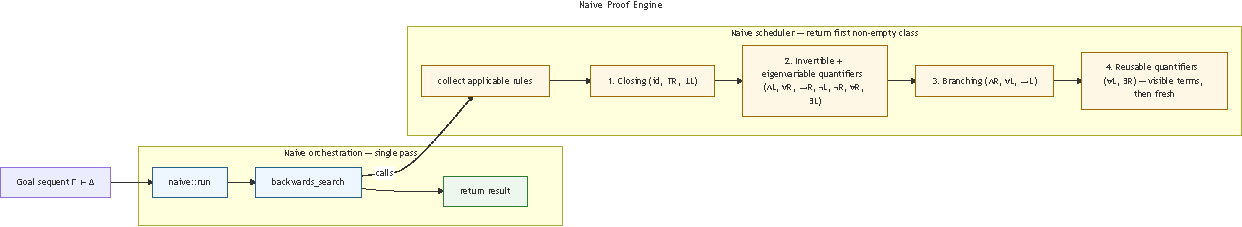
\includegraphics[width=\linewidth]{figures/naive_engine_diagram.pdf}
  \caption{Naive proof engine: single-pass DFS with the five-group
  naive scheduler.}
  \label{fig:naive-engine}
\end{figure}

\subsection{Failure Modes}\label{sec:failure}
We identify two structural weaknesses of Algorithm~\ref{alg:naive}.
\textbf{(F1) Eager eigenconstants.} Group~2 lumps the eigenvariable
quantifier rules ($\forall R$, $\exists L$) with non-branching
propositional rules, so the prover commits to a fresh eigenconstant
even when a branching propositional decomposition would have closed the
branch by identity. Each eigenconstant enlarges the symbol set, which
enlarges the candidate set for subsequent $\forall L$/$\exists R$
instantiations.
\textbf{(F2) Unbounded reusable instantiation.} Because $\forall L$ and
$\exists R$ retain the original quantified formula on the sequent,
groups~4 and 5 of Algorithm~\ref{alg:naive} permit an arbitrary number
of distinct witness terms to be tried before any sibling branch is
revisited. A na\"ive depth-first loop therefore commits to deep
instantiation chains before backtracking to easier alternatives.

At each node the backward search has branching factor $b$ (the number of
applicable rule instances), giving $O(b^d)$ nodes at proof depth $d$.
The reusable quantifier rules make $b$ grow with the size of the visible
witness pool: each fresh constant generated under (F2) enlarges this pool
for all subsequent nodes, producing super-exponential expansion in the worst
case.  First-order logic is in general undecidable~\cite{church1936entscheidungsproblem},
so a sound proof procedure must be a semi-decision procedure; on non-theorems
the prover cannot guarantee termination and instead returns \textit{Unknown}
whenever a resource bound is reached.

\subsection{Proposed Algorithm}\label{sec:proposed}

Two targeted refinements address (F1) and (F2) while leaving the shared
search kernel unchanged.

\subsubsection{Building Block A: Iterative Deepening}

Our first refinement wraps the depth-first search in an
iterative-deepening envelope~\cite{korf1985iterative}.  The outer loop
(lines 1--6 of Algorithm~\ref{alg:priority-id}) retries
\texttt{backwards\_search} from $S_0$ at increasing depth limits
$d = 1, 2, \ldots, D$, returning as soon as some depth produces a
\textsc{Provable} result.  Because proof depth is proportional to the
number of rule applications on the longest open branch, this guarantees
that every proof of depth $k$ is discovered before any branch of depth
$k{+}1$ is explored; the search never commits to a deep
quantifier-instantiation chain before exhausting all shallower
alternatives, directly mitigating (F2).

\subsubsection{Building Block B: LK$'$ Six-Class Priority Schedule}

Our second refinement replaces the five-group scheduler of
Algorithm~\ref{alg:naive} with a six-class schedule
(\textsc{PrioritySchedule} in Algorithm~\ref{alg:priority-id}).
The classes are applied in order, returning the first non-empty set of
applicable rule instances:

\begin{enumerate}
  \item \textbf{Closing rules} ($\mathit{id}$, $\top R$, $\bot L$):
    terminate the current branch immediately; no new sub-goals are created.
  \item \textbf{Non-branching propositional} ($\wedge L$, $\vee R$,
    ${\rightarrow}R$, $\neg L$, $\neg R$): invertible rules that decompose
    a connective deterministically without splitting; zero search cost.
  \item \textbf{Branching propositional} ($\wedge R$, $\vee L$,
    ${\rightarrow}L$): split the goal into multiple sub-goals without
    enlarging the term universe.
  \item \textbf{Eigenvariable quantifiers} ($\forall R$, $\exists L$):
    introduce a fresh eigenconstant.  Deferring these until after
    branching rules means propositional decomposition can close branches
    before any new symbol is added, addressing (F1).
  \item \textbf{Reusable quantifiers, visible witnesses} ($\forall L$,
    $\exists R$ instantiated with a term already on the branch):
    exhausts existing terms before generating new ones; this class is
    finite and always terminates.
  \item \textbf{Reusable quantifiers, fresh fallback} ($\forall L$,
      $\exists R$ with a freshly generated witness, subject to a
    per-occurrence budget): last resort; when the budget is exhausted
    the kernel returns \textit{Unknown} rather than \textit{NotProvable},
    preserving soundness.
\end{enumerate}

Splitting the original groups~4--5 of Algorithm~\ref{alg:naive} into
classes~5--6 means the prover always exhausts visible witnesses before
introducing a new symbol, addressing (F2).

% Requires \usepackage{algorithm} and \usepackage{algpseudocode}.
% This fragment is intended to be included from report/samplepaper.tex.

\begin{algorithm}[t]
  \caption{Priority-ID backward proof search for LK$'$}\label{alg:priority-id}
  \begin{algorithmic}[1]
    \Require Goal sequent $S_0$, maximum depth $D$, maximum steps $N$,
      timeout deadline $T$, fresh-term budget $F$
    \Ensure \textsc{Provable}, \textsc{NotProvable}, or a bounded-failure status
    \State $steps \gets 0$
    \For{$d \gets 1$ \textbf{to} $D$}
      \If{cancel requested}
        \State \Return \textsc{Cancelled}
      \EndIf
      \If{current time $\geq T$}
        \State \Return \textsc{Timeout}
      \EndIf
      \State $state \gets$ empty branch-local quantifier history
      \State $outcome \gets \Call{Search}{S_0, state, 0, d, steps, N, T, F}$
      \If{$outcome = \textsc{UnknownDepth}$}
        \State \textbf{continue}
      \Else
        \State \Return $outcome$
      \EndIf
    \EndFor
    \State \Return \textsc{UnknownDepth}

    \Function{Search}{$S, state, depth, limit, steps, N, T, F$}
      \If{cancel requested}
        \State \Return \textsc{Cancelled}
      \EndIf
      \If{current time $\geq T$}
        \State \Return \textsc{Timeout}
      \EndIf
      \If{$depth > limit$}
        \State \Return \textsc{UnknownDepth}
      \EndIf
      \If{$steps \geq N$}
        \State \Return \textsc{UnknownSteps}
      \EndIf
      \State $steps \gets steps + 1$
      \State $R \gets \Call{PrioritySchedule}{S, state, F}$
      \If{$R = \emptyset$}
        \State \Return \textsc{NotProvable}
      \EndIf
      \If{$R = \textsc{QuantifierExhausted}$}
        \State \Return \textsc{UnknownQuantifierBudget}
      \EndIf
      \State $best \gets \textsc{NotProvable}$
      \ForAll{scheduled rule $r \in R$}
        \State $state' \gets state$
        \If{$r$ instantiates $\forall L$ or $\exists R$ with term $t$}
          \State record $(r.occurrence, t, r.isFresh)$ in $state'$
        \EndIf
        \State $app \gets$ apply $r$ backwards to $S$
        \If{$app$ closes the branch}
          \State \Return \textsc{Provable}
        \ElsIf{$app$ produces premises $P_1,\ldots,P_k$}
          \ForAll{$P_i$ in order}
            \State $child \gets \Call{Search}{P_i, state', depth+1, limit, steps, N, T, F}$
            \If{$child \neq \textsc{Provable}$}
              \State $best \gets \Call{MergeOutcome}{best, child}$
              \State \textbf{break}
            \EndIf
          \EndFor
          \If{all premises returned \textsc{Provable}}
            \State \Return \textsc{Provable}
          \EndIf
        \Else
          \State $best \gets \Call{MergeOutcome}{best, app.status}$
        \EndIf
        \If{$best$ is \textsc{Timeout} or \textsc{Cancelled}}
          \State \Return $best$
        \EndIf
      \EndFor
      \State \Return $best$
    \EndFunction

    \Function{PrioritySchedule}{$S, state, F$}
      \State $M \gets$ all structurally applicable LK$'$ rule matches in $S$
      \State return the first non-empty class from the following ordered list:
      \Statex \hspace{1em}1. $id$, $\top R$, $\bot L$
      \Statex \hspace{1em}2. $\wedge L$, $\vee R$, $\rightarrow R$, $\neg L$, $\neg R$
      \Statex \hspace{1em}3. $\wedge R$, $\vee L$, $\rightarrow L$
      \Statex \hspace{1em}4. $\forall R$, $\exists L$
      \Statex \hspace{1em}5. $\forall L$, $\exists R$ using unused visible branch terms
      \Statex \hspace{1em}6. $\forall L$, $\exists R$ using one fresh fallback term if $F$ permits
      \If{a reusable quantifier matched but classes 5 and 6 are empty}
        \State \Return \textsc{QuantifierExhausted}
      \EndIf
      \State \Return $\emptyset$
    \EndFunction
  \end{algorithmic}
\end{algorithm}


\subsection{Combined Prover}\label{sec:combined}

The proposed prover \texttt{priority-id} combines both building blocks:
the six-class priority schedule is injected into \texttt{backwards\_search},
which is then wrapped in the iterative-deepening outer loop.  Two control
engines are included for comparison: \texttt{id}, which pairs iterative
deepening with the naive scheduler to isolate the effect of depth-bounding,
and \texttt{naive}, the unmodified baseline.

Figure~\ref{fig:priority-id-engine} shows the composition of the two
building blocks: the iterative-deepening envelope drives the outer search
strategy, while the six-class LK$'$ priority scheduler governs which rules
are attempted at every node inside the shared \texttt{backwards\_search}
kernel.

\begin{figure}[t]
  \centering
  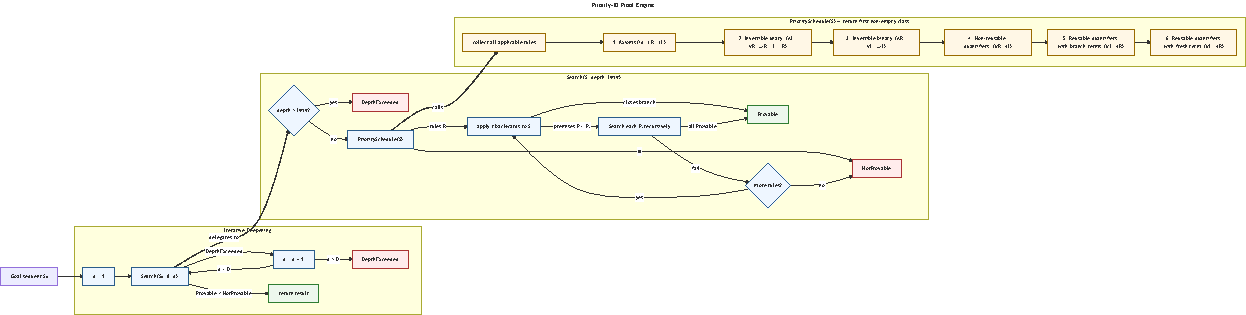
\includegraphics[width=\linewidth]{figures/priority_id_engine_diagram.pdf}
  \caption{Priority-ID proof engine: iterative-deepening envelope around
  \texttt{backwards\_search} with the six-class LK$'$ priority scheduler.}
  \label{fig:priority-id-engine}
\end{figure}

\subsection{Expected Performance}\label{sec:hypothesis}

We expect (F2) to be the dominant failure mode on provable benchmarks.
TPTP provable problems frequently admit proofs at shallow depth, but the
naive DFS commits to groups~4--5 quantifier instantiation before exhausting
branching alternatives at the same level.  Each fresh witness widens the
search tree (branching factor $b$ grows with the witness pool), and since
the tree has $O(b^d)$ nodes at depth $d$, even moderate instantiation depth
exhausts the time budget before backtracking reaches a shorter proof.
Iterative deepening corrects this: by bounding depth at $d = 1, 2, \ldots$
in sequence, the search explores the $O(b^d)$ tree at the current limit
before allowing any depth-$d{+}1$ branch, guaranteeing that a proof of
depth $k$ is found on iteration $k$.  The \texttt{id} engine should therefore
account for the majority of additional solves.

The six-class schedule addresses (F1), which compounds (F2): each premature
eigenconstant enlarges the visible-term pool, widening the $\forall L$/$\exists
R$ candidate set for all subsequent iterations and slowing each deepening pass.
Delaying eigenvariable introduction to after branching propositional rules
(class 4 vs.\ group 2) reduces this widening.  The visible-first/fresh-fallback
split of classes~5--6 provides a further tightening: the prover stays within
the current term universe as long as possible, deferring symbol creation to
when it is strictly necessary.

Together, both refinements should yield strictly more solves than either
building block alone, with iterative deepening contributing the larger share
and the priority schedule providing a consistent additional gain on problems
with many quantified atoms.

\section{Implementation and Experiment}\label{sec:implementation}

\subsection{Implementation}

The prover is written in Rust~\cite{rust2024} (edition~2024) and consists
of approximately 4{,}500 lines of source code spread over a parser,
abstract-syntax tree, sequent representation, rule applicators, search
engine, and a CLI front-end. The parser is built with
\texttt{pest}~\cite{pest2024}, a parsing-expression-grammar generator,
against a hand-written grammar for the first-order-form (FOF) fragment of
the TPTP language~\cite{Sut17}. The CLI uses
\texttt{clap}~\cite{clap2024} for argument parsing and
\texttt{rusqlite}~\cite{rusqlite2024} for persisting per-problem results
to a SQLite database. Cancellation under \texttt{Ctrl+C} is handled by the
\texttt{ctrlc} crate. The three search engines (\texttt{naive},
\texttt{id}, \texttt{priority-id}) are selected at the command line and
share all code outside the rule scheduler.

Figure~\ref{fig:naive-engine} shows the call structure of the naive
engine.

\begin{figure}
  \centering
  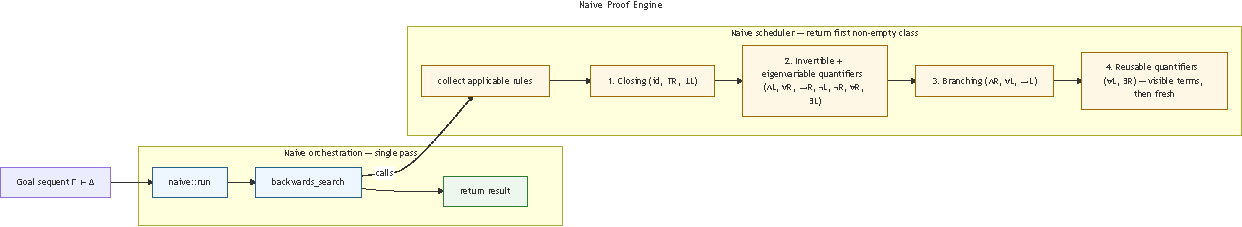
\includegraphics[width=\linewidth]{figures/naive_engine_diagram.pdf}
  \caption{Call structure of the naive proof engine.}
  \label{fig:naive-engine}
\end{figure}

Two design points warrant mention. First, the LK$'$-reusable rules
$\forall L$ and $\exists R$ retain the original quantified formula on its
side of the sequent after instantiation, so the prover tracks per-branch
quantifier-instantiation history (which terms have been used for which
quantified occurrence) to avoid trying the same instantiation twice on the
same branch. Second, fresh-name generation for both eigenconstants
($\forall R$, $\exists L$) and fallback witnesses ($\forall L$, $\exists R$)
inspects every symbol currently visible in the sequent and returns a name
not in that set, guaranteeing eigenvariable freshness without further
$\alpha$-renaming machinery. Substitution is capture-avoiding by
construction because only ground terms are ever instantiated for bound
variables.

\subsection{Experimental Setup}

All benchmarks were run on a single machine: Windows~11 Home
(Version~10.0.26200, Build~26200), Intel Core Ultra~7~258V (8~cores,
x86-64), 32\,GB RAM, Rust~1.85. Each prover invocation was given a
1{,}000\,ms wall-clock timeout, a recursive search-depth limit of 128, and
a fresh-fallback budget of one term per quantified occurrence. For the TPTP
and FOLIO datasets a step limit of 10{,}000 rule applications was also
imposed. For the synthetic dataset the step limit was set to effectively
unlimited (10$^{11}$), with the wall-clock timeout as the sole binding
resource constraint; an initial run with 10{,}000 steps produced too few
decisions on synthetic problems to be informative, so the limit was
raised. Problems whose non-comment biconditional
($\Leftrightarrow$) count exceeds six are skipped before parsing; this cap
prevents large biconditional chains from consuming proof-search resources
disproportionate to the rest of the benchmark. Results were persisted to SQLite databases; the analysis pipeline
(Python~3.12 with \texttt{pandas} and \texttt{matplotlib}) loads all
results directly, as each database contains exactly one run per engine at
identical parameter settings.

\subsection{Datasets}

Three datasets are used, covering standard ATP benchmarks,
natural-language-derived problems, and synthetic controlled problems.

\subsubsection{TPTP.}
Two subsets of the TPTP problem library~\cite{Sut17} are used. The first is a
737-problem provable subset (FOF/THM), restricted to problems with 0--50 input
formulae, 0--150 atoms, and no equality or arithmetic. The second is a
204-problem counter-satisfiable subset (FOF/CSA) drawn from the same
complexity bounds, in which each problem is known to have no proof because
its negation is satisfiable. The two subsets together test both sides
of the prover against problems with
known status across diverse mathematical domains.

\subsubsection{FOLIO.}
The FOLIO dataset~\cite{han2024folio} provides 280 human-authored
natural-language reasoning problems formalised as FOF, testing whether the
prover's behaviour generalises beyond the controlled TPTP filter.

\subsubsection{Synthetic.}
202 synthetic FOF problems were generated programmatically across four tiers,
\emph{easy} (32), \emph{medium} (60), \emph{hard} (60), \emph{expert}
(50), with proof depth $n\in[2,15]$ and distractor count $d\in[0,14]$
scaling jointly with tier. Four problem families are used.
\textbf{Implication chains}: a conjecture reachable from a ground fact via
$n$ universally quantified steps, with $d$ structurally identical
distractor axioms. \textbf{Syllogisms}: a fixed class hierarchy with a
ground instance for one individual. \textbf{Transitivity chains}: a single
binary transitivity axiom plus ground edge facts, requiring repeated reuse
of the same axiom across different instantiations.
\textbf{Quantifier alternation}: single-formula conjectures testing
classical $\forall$/$\exists$ theorems and non-theorems. Unprovable
variants negate the conjecture (e.g., remove a chain link, change the
syllogism individual, or ask for an unreachable node).


\subsection{Results}

A problem is \emph{decided} when the prover returns \textit{Provable} or
\textit{NotProvable}, as opposed to timing out or hitting a resource bound.
Table~\ref{tab:summary} reports decided counts across all datasets.

\begin{table}[t]
  \centering
  \caption{Decided problems per engine across all datasets
  (timeout 1{,}000\,ms, depth 128, fresh-fallback budget 1;
  steps 10{,}000 for TPTP and FOLIO, effectively unlimited for synthetic).
  A problem is \emph{decided} when the prover returns \textit{Provable}
  or \textit{NotProvable}.}
  \label{tab:summary}
  \begin{tabular}{lrrrr}
    \toprule
    Engine & TPTP (888) & FOLIO (280) & Synthetic (202) & Total (1370) \\
    \midrule
    \texttt{naive}       & 156 (17.6\,\%) & 57 (20.4\,\%) & 26 (12.9\,\%) & 239 (17.4\,\%) \\
    \texttt{id}          & 203 (22.9\,\%) & 57 (20.4\,\%) & 39 (19.3\,\%) & 299 (21.8\,\%) \\
    \texttt{priority-id} & 213 (24.0\,\%) & 66 (23.6\,\%) & 42 (20.8\,\%) & 321 (23.4\,\%) \\
    \bottomrule
  \end{tabular}
\end{table}

\begin{figure}[h]
  \centering
  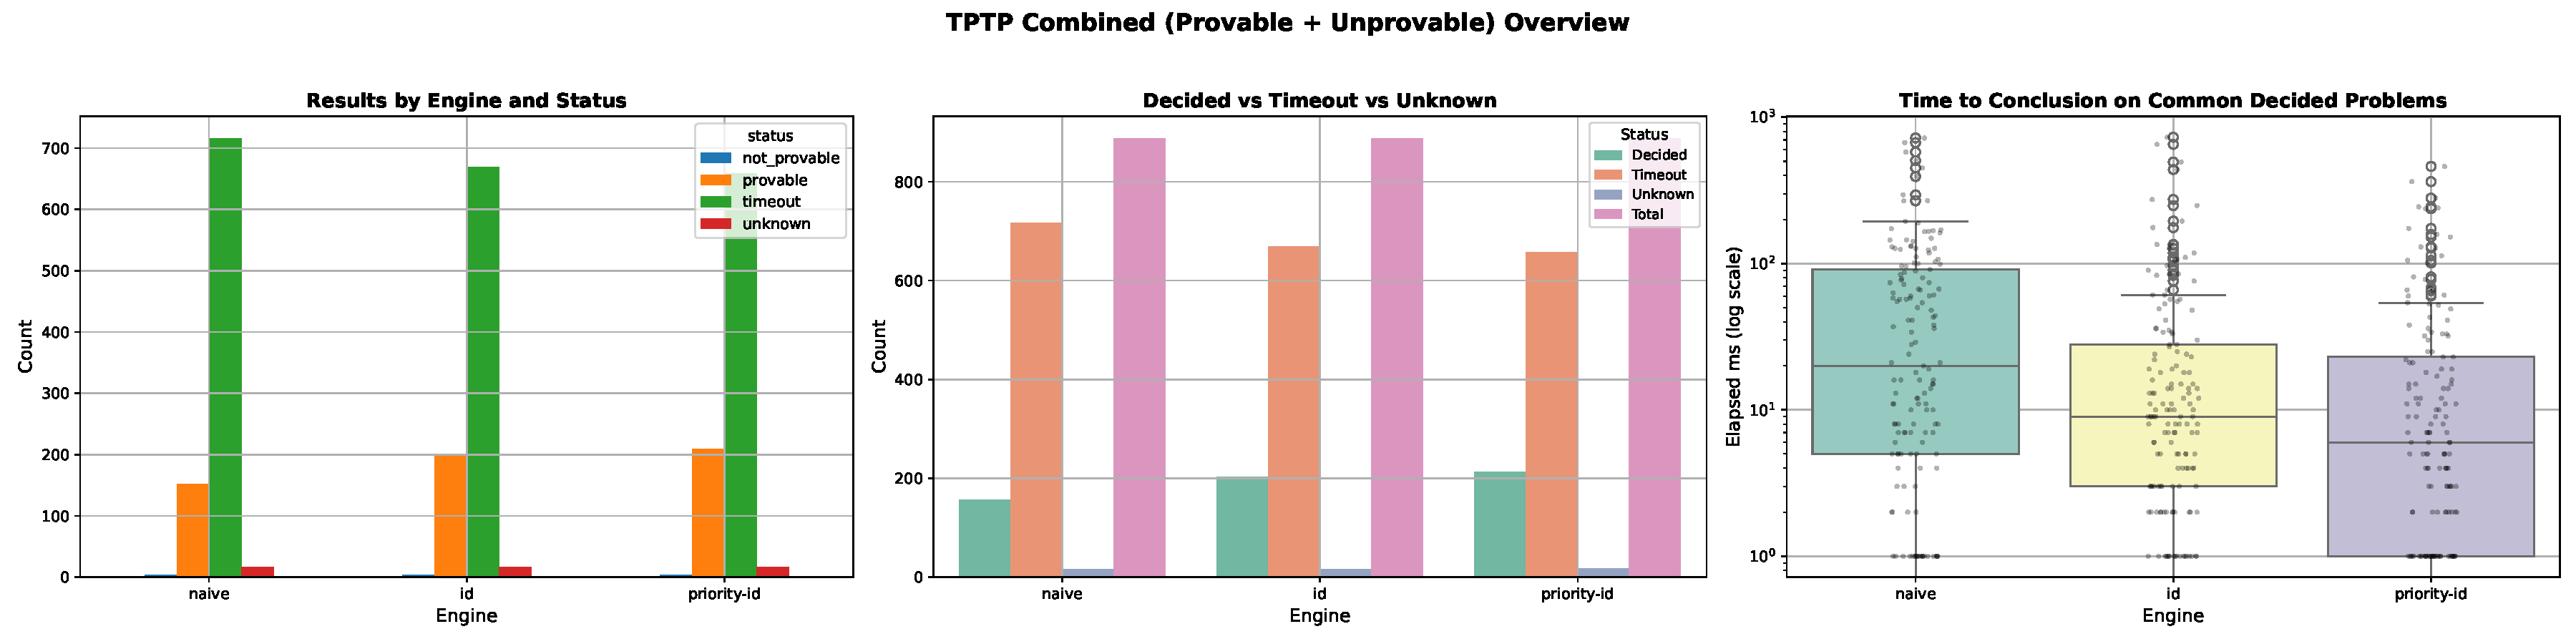
\includegraphics[width=\linewidth]{figures/tptp_combined_overview.pdf}
  \caption{TPTP combined dataset (888 problems): outcome counts by engine
    (left), decided vs.\ timeout vs.\ unknown breakdown (centre), and
    time to conclusion on commonly decided problems, log scale (right).}
  \label{fig:tptp-overview}
\end{figure}

\begin{figure}[h]
  \centering
  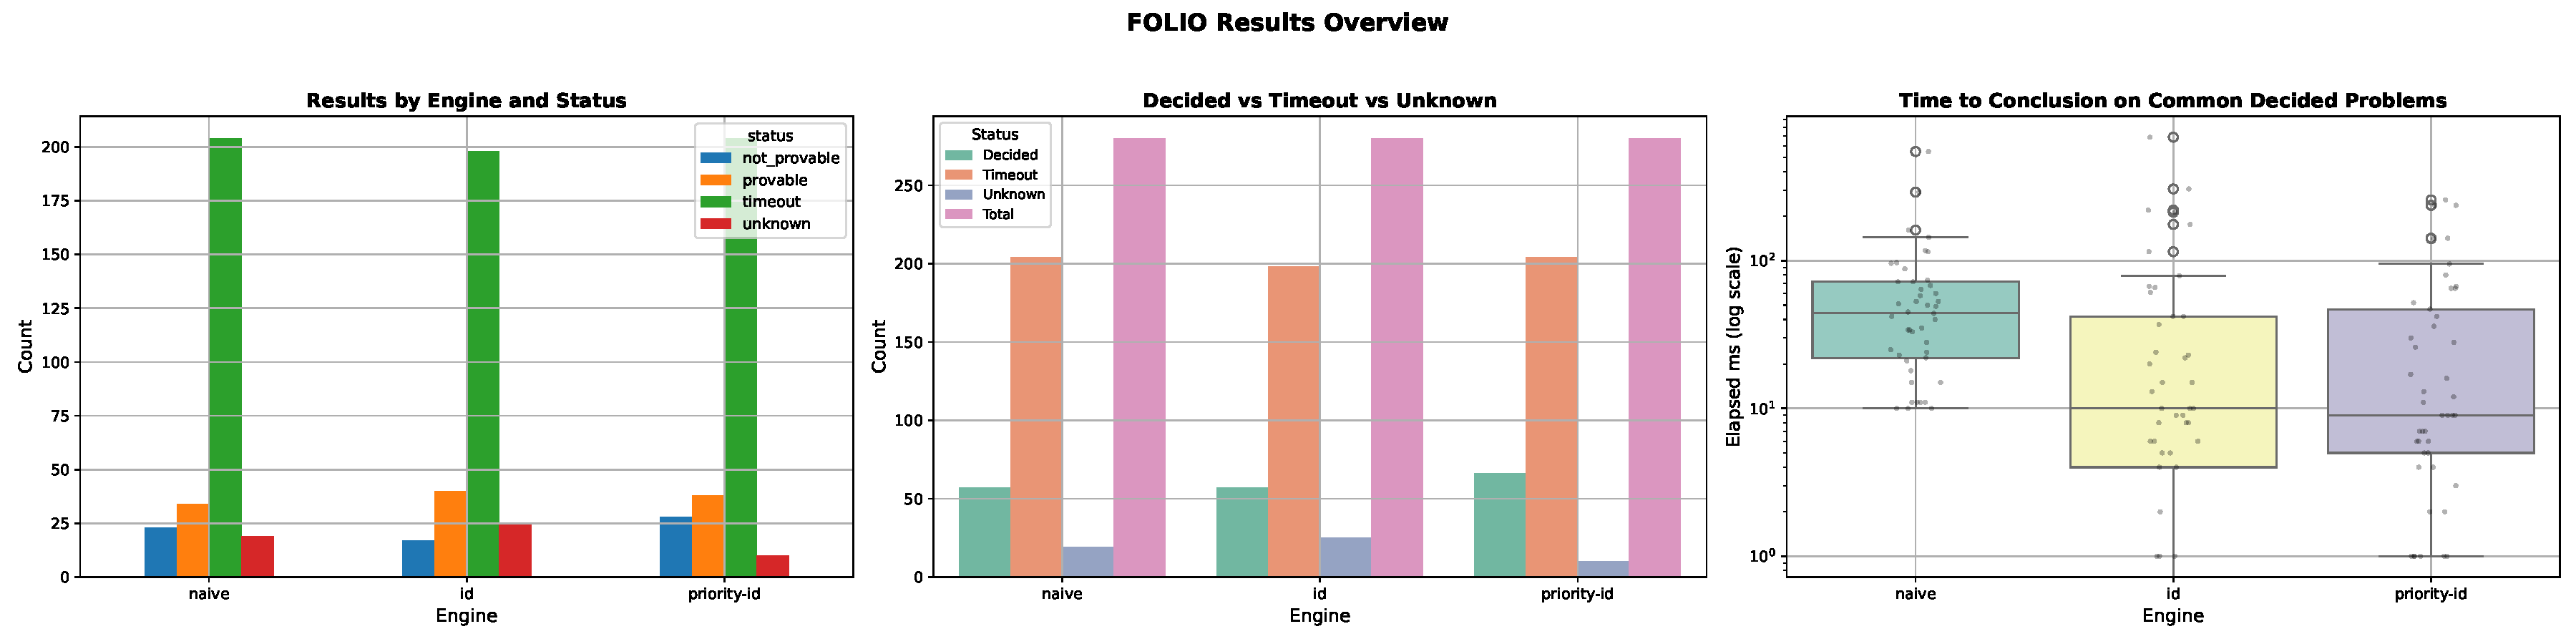
\includegraphics[width=\linewidth]{figures/folio_overview.pdf}
  \caption{FOLIO validation set (280 problems): same layout as
    Fig.~\ref{fig:tptp-overview}.}
  \label{fig:folio-overview}
\end{figure}

\begin{figure}[h]
  \centering
  \includegraphics[width=\linewidth]{figures/ai_generated_overview.pdf}
  \caption{Synthetic dataset (202 problems): same layout as
    Fig.~\ref{fig:tptp-overview}.}
  \label{fig:ai-overview}
\end{figure}

On the TPTP benchmark (Figure~\ref{fig:tptp-overview}), \texttt{naive}
decides 156 problems, \texttt{id} decides 203 ($+30\,\%$), and
\texttt{priority-id} decides 213 ($+37\,\%$ over \texttt{naive}). All
additional solves come from the provable subset; the four
counter-satisfiable decisions are shared by all three engines. The
log-scale timing panel shows that \texttt{id} and \texttt{priority-id}
not only solve problems \texttt{naive} cannot reach, but also solve the
shared problems faster on average, reflecting fewer wasted steps in
dead-end branches.

The FOLIO results (Figure~\ref{fig:folio-overview}) reveal a different
pattern. \texttt{naive} and \texttt{id} both decide 57 problems, but with
a shifted composition: \texttt{naive} returns 34~\textit{Provable} and
23~\textit{NotProvable}, while \texttt{id} returns 40~\textit{Provable}
and 17~\textit{NotProvable}. These are not the same problems. \texttt{id}
finds 11 proofs that \texttt{naive} timed out on, but loses 5 proofs that
\texttt{naive} found: iterative deepening's repeated restarts exhaust
the step budget before those branches close. Simultaneously, \texttt{id}
converts 6 of \texttt{naive}'s \textit{NotProvable} decisions to
\textit{Unknown}: the restarts prevent the search from fully exhausting
those spaces, so problems \texttt{naive} certified as unprovable become
undecided under \texttt{id}. The net result is a coincidental wash at 57
decided problems. \texttt{priority-id} resolves this trade-off by spending
fewer steps per iteration on unproductive branches. It decides 66
problems (38~\textit{Provable} and 28~\textit{NotProvable}), converting
11 of \texttt{id}'s \textit{Unknown} and \textit{Timeout} outcomes to
\textit{NotProvable} (the more disciplined step budget allows those
search spaces to be fully exhausted), and reducing \textit{Unknown} from
25 to 10.

On the synthetic dataset (Figure~\ref{fig:ai-overview}), \texttt{naive}
decides 26 problems, \texttt{id} decides 39 ($+50\,\%$ over
\texttt{naive}), and \texttt{priority-id} decides 42 ($+62\,\%$ over
\texttt{naive}). The tier breakdown
(Figure~\ref{fig:synthetic-tier}, Table~\ref{tab:synthetic-tier}) shows
where these gains arise. On medium-tier problems \texttt{naive} decides
10 of 60, \texttt{id} decides 19, and \texttt{priority-id} decides 20.
On hard-tier problems \texttt{naive} decides none, while \texttt{id} and
\texttt{priority-id} decide 3 and 5 respectively. No engine decides any
expert-tier problem. The gains are concentrated in implication-chain and
syllogism families; all 43 transitivity-chain problems are unsolved by
every engine: every invocation times out, as the repeated-reuse proof
strategy required by those problems does not terminate within the
1{,}000\,ms wall-clock limit.
Figure~\ref{fig:synthetic-depth} plots solve rate against chain depth for
implication-chain problems, confirming that \texttt{naive}'s solve rate
collapses beyond depth~4 while \texttt{id} and \texttt{priority-id}
maintain non-zero solve rates into the hard tier. This is the controlled
signature of F2: the naive DFS descends into distractor-quantifier chains
at every step, making chain depth the dominant cost factor, while
iterative deepening recovers the short proofs that DFS bypasses. All
three engines agree on all four \textit{NotProvable} decisions.

\begin{figure}[h]
  \centering
  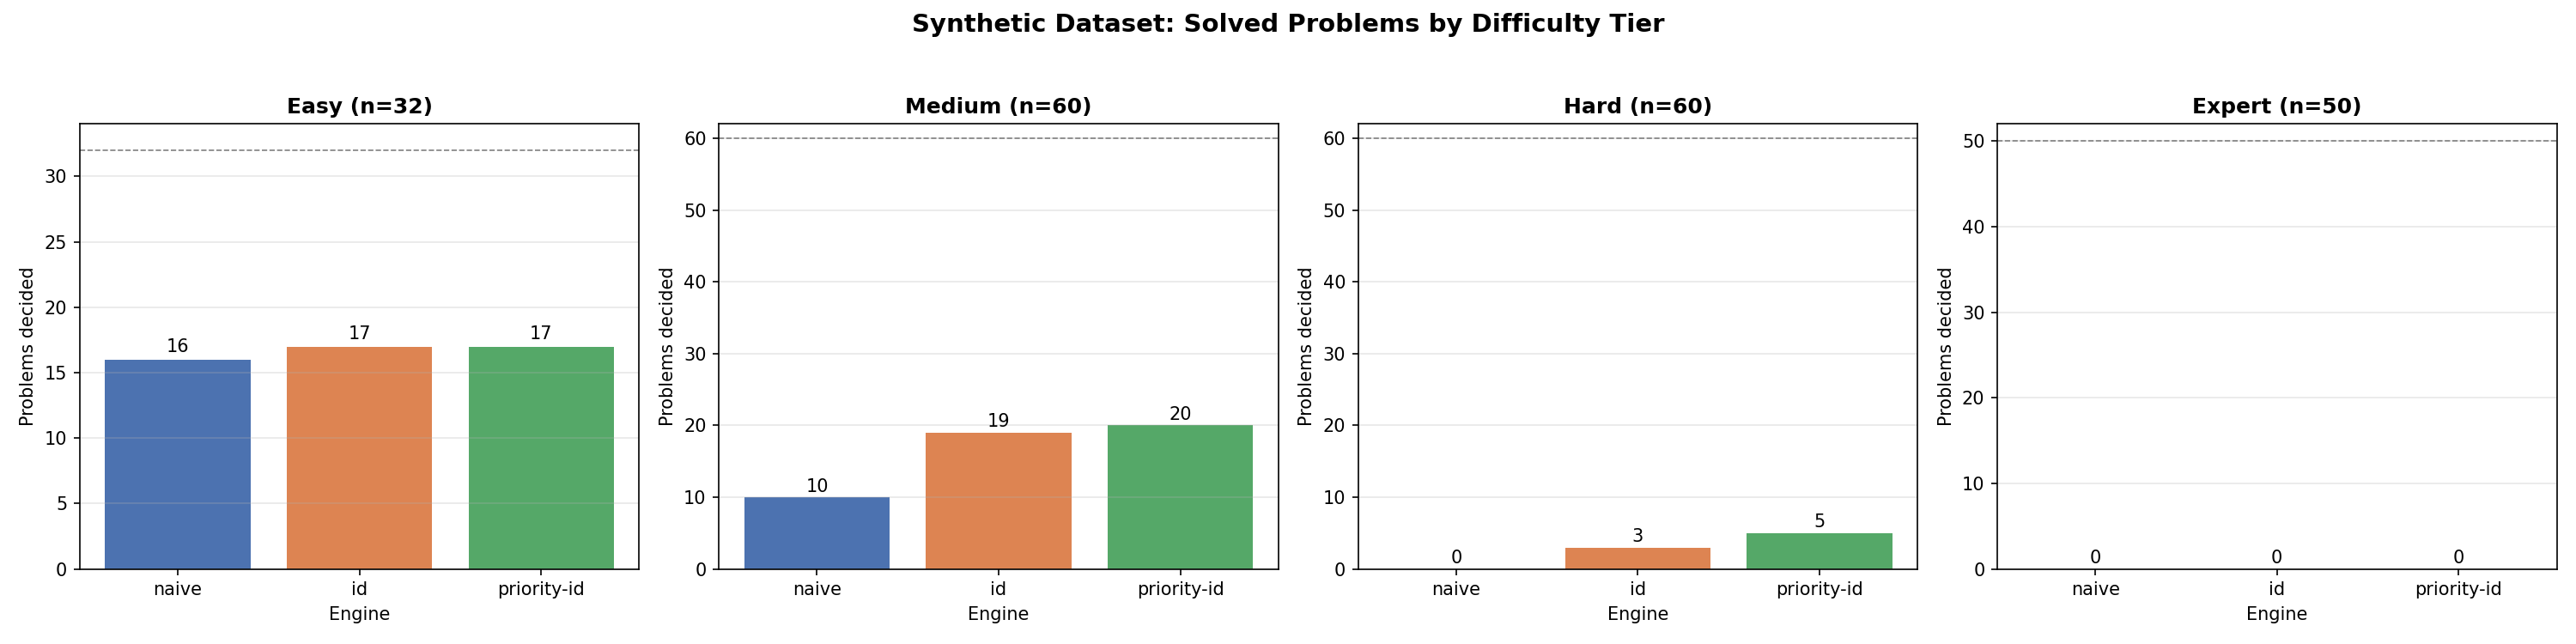
\includegraphics[width=\linewidth]{figures/ai_generated_tier_breakdown.pdf}
  \caption{Synthetic dataset (202 problems): decided problems per engine
    at each difficulty tier. The dashed line marks the total number of
    problems in that tier.}
  \label{fig:synthetic-tier}
\end{figure}

\begin{figure}[h]
  \centering
  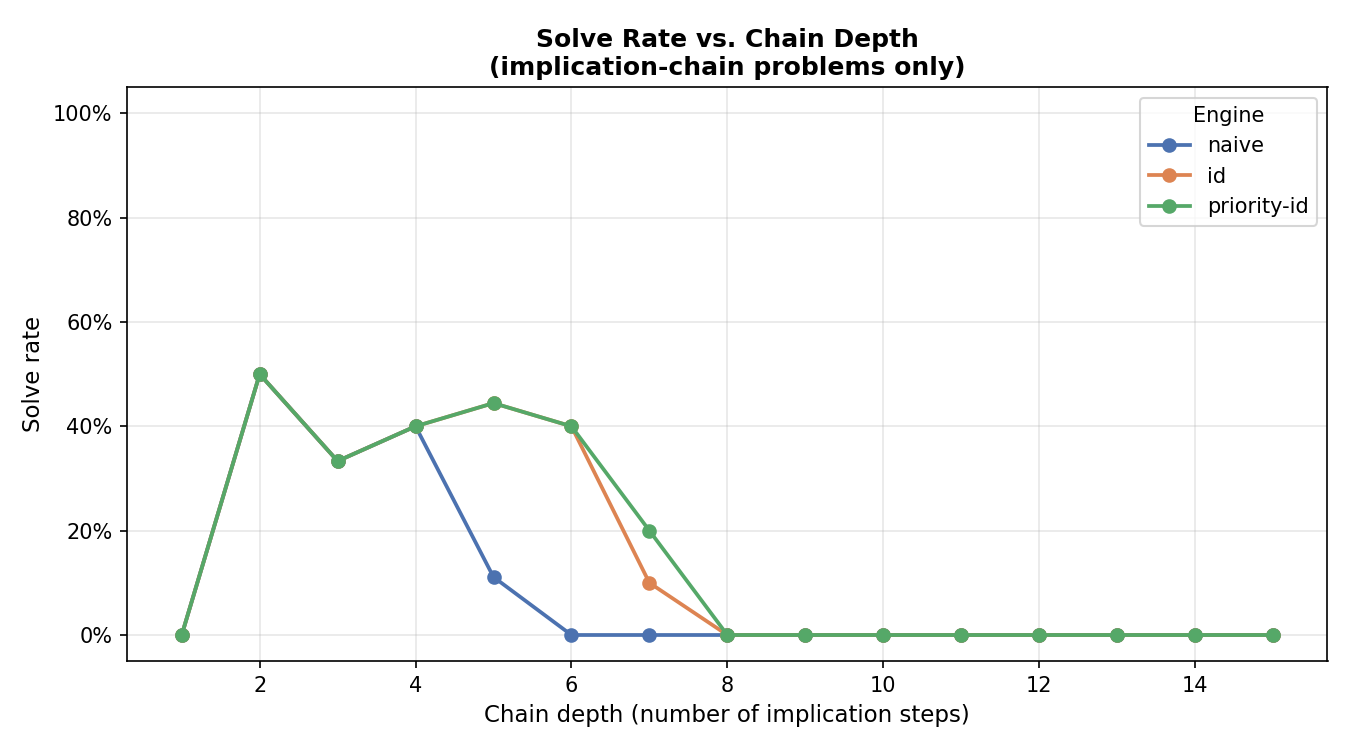
\includegraphics[width=0.85\linewidth]{figures/ai_generated_depth_solve_rate.pdf}
  \caption{Solve rate vs.\ chain depth for implication-chain problems.
    Each point is the fraction of problems at that depth decided by the
    engine; depth is the number of $\forall L$ steps required.}
  \label{fig:synthetic-depth}
\end{figure}

Across all datasets the two refinements are consistently additive.
Iterative deepening provides the larger gain on TPTP and synthetic
problems, where shallow proofs exist but are blocked by deep quantifier
instantiation. The priority schedule drives the net improvement on FOLIO,
where its more disciplined use of the step budget converts undecided
problems into definitive outcomes. Per-dataset breakdowns by outcome type
are given in Appendix~\ref{app:tables}.

